\documentclass[letterpaper,10pt]{article}
\usepackage[top=2cm, bottom=1.5cm, left=1cm, right=1cm]{geometry}
\usepackage{amsmath, amssymb, amsthm,graphicx}
\usepackage{fancyhdr}
\pagestyle{fancy}

\lhead{\today}
\chead{QE Assignment 9}
\rhead{Justin Hood}

\newcommand{\Z}{\mathbb{Z}}
\newcommand{\Q}{\mathbb{Q}}
\newcommand{\R}{\mathbb{R}}
\newcommand{\C}{\mathbb{C}}
\newtheorem{lem}{Lemma}

\begin{document}
\begin{enumerate}
\item To begin, we consider the steering wheel data. We first compute our standard $\bar{X}$ and $R$ charts for the process. Using Excel, we find the charts below,
\begin{center}
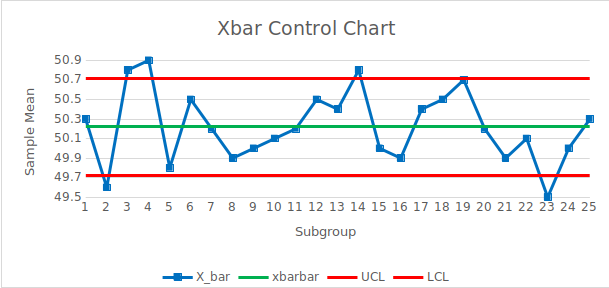
\includegraphics[scale=1]{1a.png}
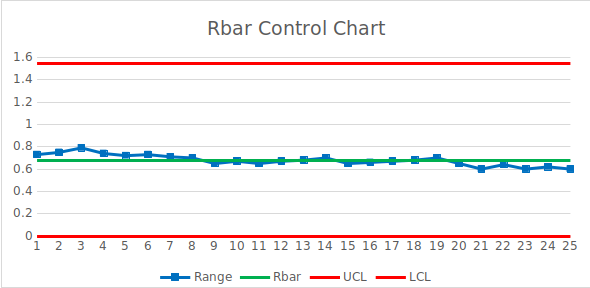
\includegraphics[scale=1]{1b.png}
\end{center}
From this, we clearly see that the process is not within control, as there are several points on the $\bar{X}$ chart that are not within our LCL-UCL boundary. Using conditional formatting, we isolate the extrema subgroups to be, $\{2,3,4,14,23\}$. We assume that assignable causes are known for these cases, and remove these data points from the table, and recompute. The new $\bar{X}$ chart follows,
\begin{center}
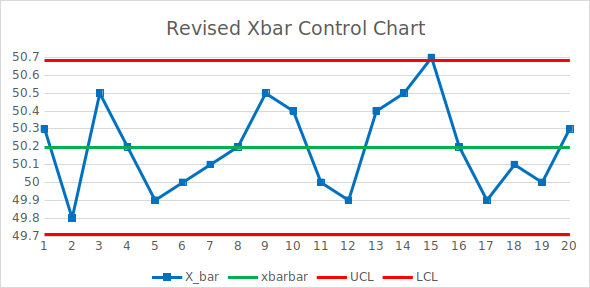
\includegraphics[scale=1]{1c.png}
\end{center}
We now have a new control chart that still has one point outside of control. As such, we see that the process is probably not in control. If we assume again that we can find an assignable cause for this extrema, we may remove this point to achieve the following chart,
\begin{center}
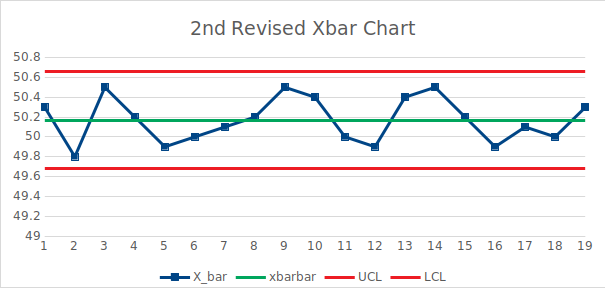
\includegraphics[scale=1]{1d.png}
\end{center}
This final chart appears to be within control. We see that outside of the cases that we have assignable causes for, the process is close to in control, but given the high percentage of erroneous points due to the causes, the process should probably be evaluated for improvement possibilities.  For a process that we desire to have a mean of $50.0$, we see that this process has a mean slightly higher than $50$, so steps should likely be taken to reduce the mean to $50$.
\item We now consider the data from the Case 7 chart.  We first compute the $R$ chart components as before, resulting in this chart,
\begin{center}
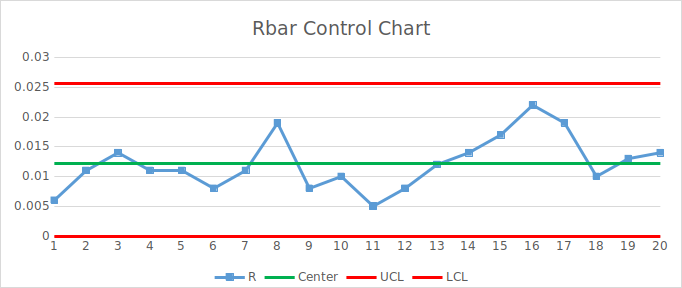
\includegraphics[scale=1]{2a.png}
\end{center}
Seeing as there are no major discrepancies in the R chart, we consider the $\bar{X}$ values. From a basic inspection, we see that there is a positive trend to the data. So, we look at the scatter plot for the linear trend equation in the $\bar{X}$ data.
\begin{center}
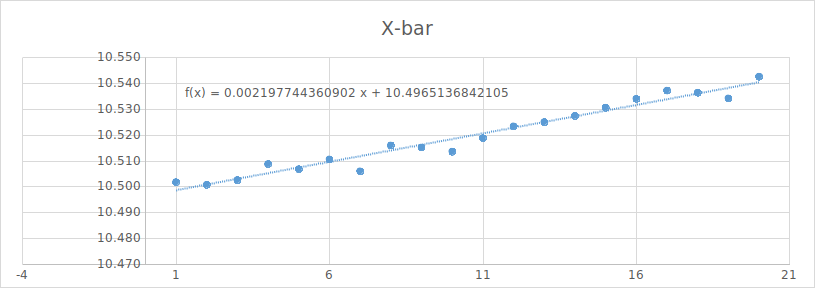
\includegraphics[scale=.8]{2b.png}
\end{center}
We see now that there is a neat linear trend in the data, with the formula,
\[y=10.49651+0.002198x\]
So, we construct the sloped $\bar{X}$ control chart below,
\begin{center}
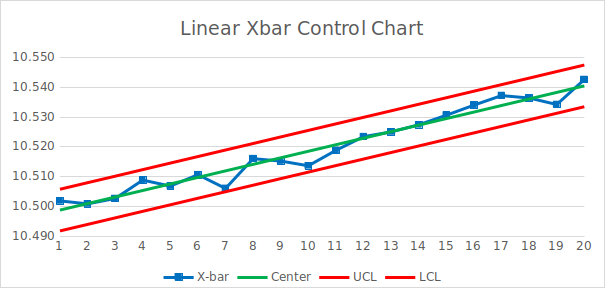
\includegraphics[scale=1]{2c.png}
\end{center}
With this sloped equation, we see that the process is within control. This, however, is predicated on the assumption that the drift in the data is acceptable for the process.
\item We now consider the keyhole brake data. Using a moving range with $n=2$, we construct the $X$ charts for both keyholes. The results follow,
\begin{center}
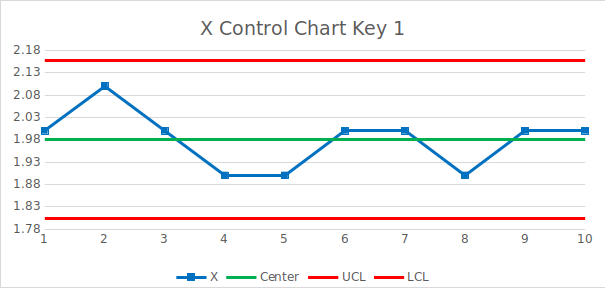
\includegraphics[scale=1]{3a.png}
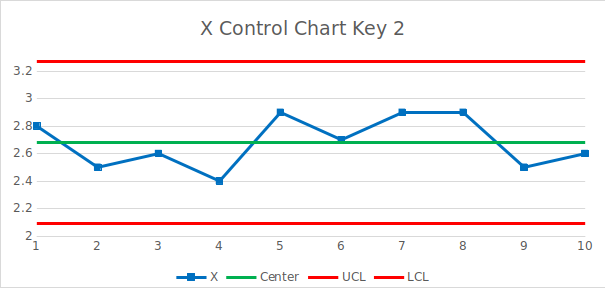
\includegraphics[scale=1]{3b.png}
\end{center}
We see that while both processes are within control, there are significant differences between the two keyholes. First, $Center_1=1.98$ and $Center_2=2.68$. So, we see that there is a difference $0.7$ between the two key centers. Given that this difference is over $20\%$ of the center value, we conclude that these positions are distinctly different. We also see that the width of the control limits are significantly different, with the smaller width being for keyhole one. Assuming that the process for producing the keyholes is the same, we might consider looking at process 2 to reduce the variance in the process to similar values to process 1.
\item Finally, we consider the MPG data. As before, we must construct the $X$ chart, but we shall use $n=3$ for our moving range calculation. The results are,
\begin{center}
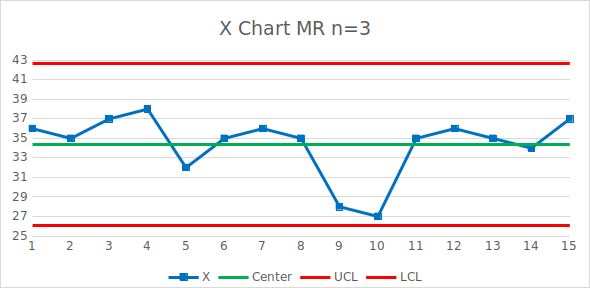
\includegraphics[scale=1]{4a.png}
\end{center}
This chart shows that the process appears to be in control, with perhaps an irregularity around the 9th or 10th measurement that could warrant further investigation.
\end{enumerate}
\end{document}
